\section{Results}
This project was mostly exploratory; we envision a previously unaddressed type of intermittent bug that can theoretically exist, develop a static analysis tool to detect the relevant code pattern, and then see if compelling examples actually exist in the wild. They do, particularly in sensor drivers and low-level client applications. For our results, we present three case studies: one taken from the TI-RTOS magnetometer driver, and two taken from example software applications bundled with TI-RTOS. For each case, we give the simplified source code, annotated with a restart and power failure point that triggers the bug, the program execution trace, and a discussion of the possible consequences of each bug.

\subsection{The Magnetometer Driver}

Figure \ref{fig:mag} shows the initialization function of the magnetometer driver, with the simplfied source code on the right, and the buggy execution trace on the left. The function checks that the sensor is powered on and conditionally reads from the I2C bus. If the read was successful, the raw data from the bus read is stored into the X, Y, Z fields of the calibration structure, and if the read was not successful the function simply returns. 
\begin{figure}[h]
\centering
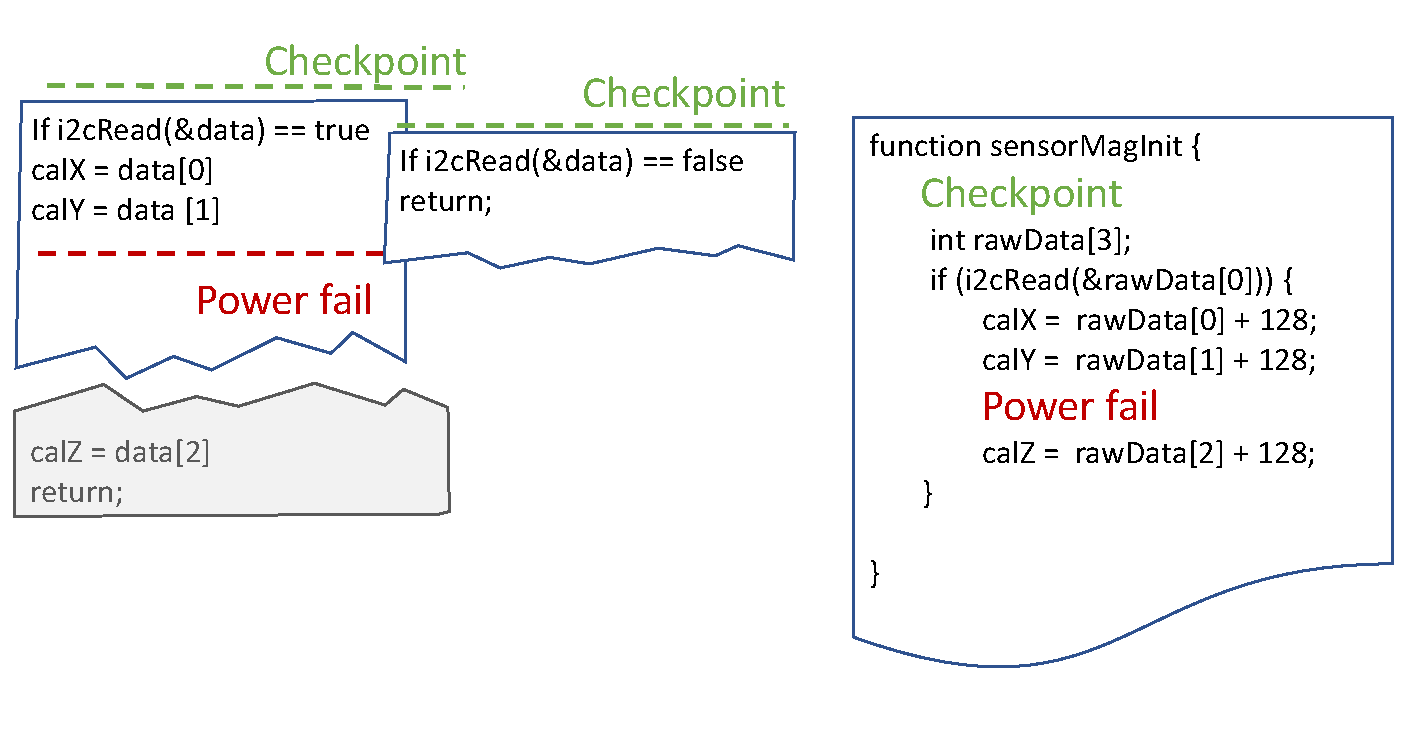
\includegraphics[width=1\columnwidth]{maginit_bug.pdf}
\caption{Bug in magnetometer initialization. Power failing while updating the calibration fields can cause the calibration data to become inconsistent, corrupting any future magnetometer reads that use the calibration.}
\label{fig:mag}
\end{figure}

Non-idempotent I/O enters the program at the I2C read, from both the return value and the actual raw data, and in this case the program branches on the return value. A buggy execution is possible if we latch execution state at the beginning of the function and read successfully from the bus. Since the read returned true, we take the branch, and begin storing the raw data into the calibration fields. In this particular execution, the device runs out of power and fails after writing to calY. The write to calZ, in the greyed-out portion of the trace, is not reached. On reboot, execution resumes from the top of the function, but on this execution the read from the bus fails, introducing the I/O non-idempotency into the program. The branch is not taken, and the function returns, leaving the calibration data in a state unreachable on continuous execution - two fields are set with the correct data, but the third has some unknown default value. 
Since this is a device driver, any higher level applications that read data from the magnetometer will filter it through these corrupted, inconsistent calibration fields, possibly leading to wildly incorrect application behavior or crashes.  

\subsection{Wireless Sensor Node Concentrator}
\begin{figure}[h]
\centering
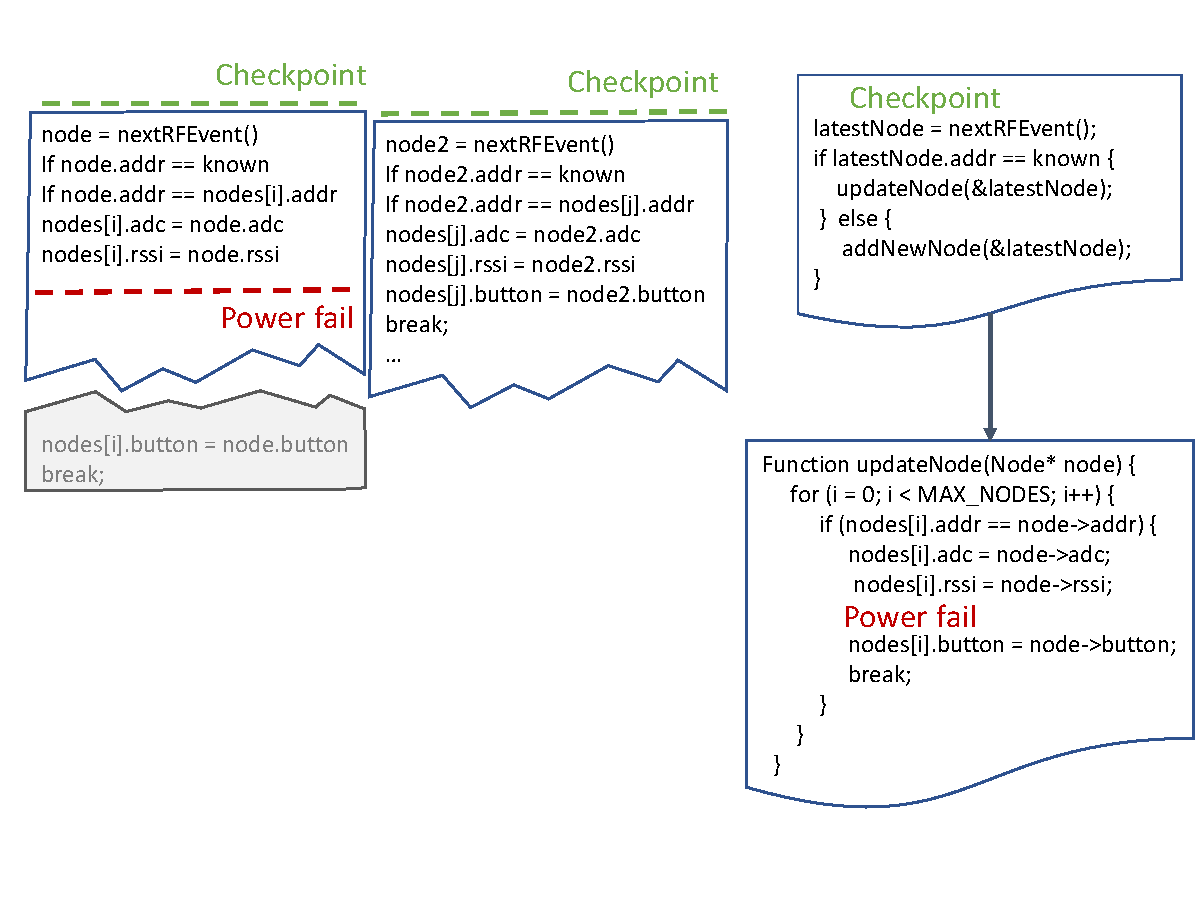
\includegraphics[width=1\columnwidth]{wsn_concentrator_bug.pdf}
\caption{Bug in WSN concentrator. Power failing while updating the node structure can cause the node list to become inconsistent, corrupt the payload ("button" field) or use out-of-date timing information, possibly messing up system protocols}
\label{fig:wsn}
\end{figure}

\subsection{RF EasyLink Receiver}
\begin{figure}[h]
\centering
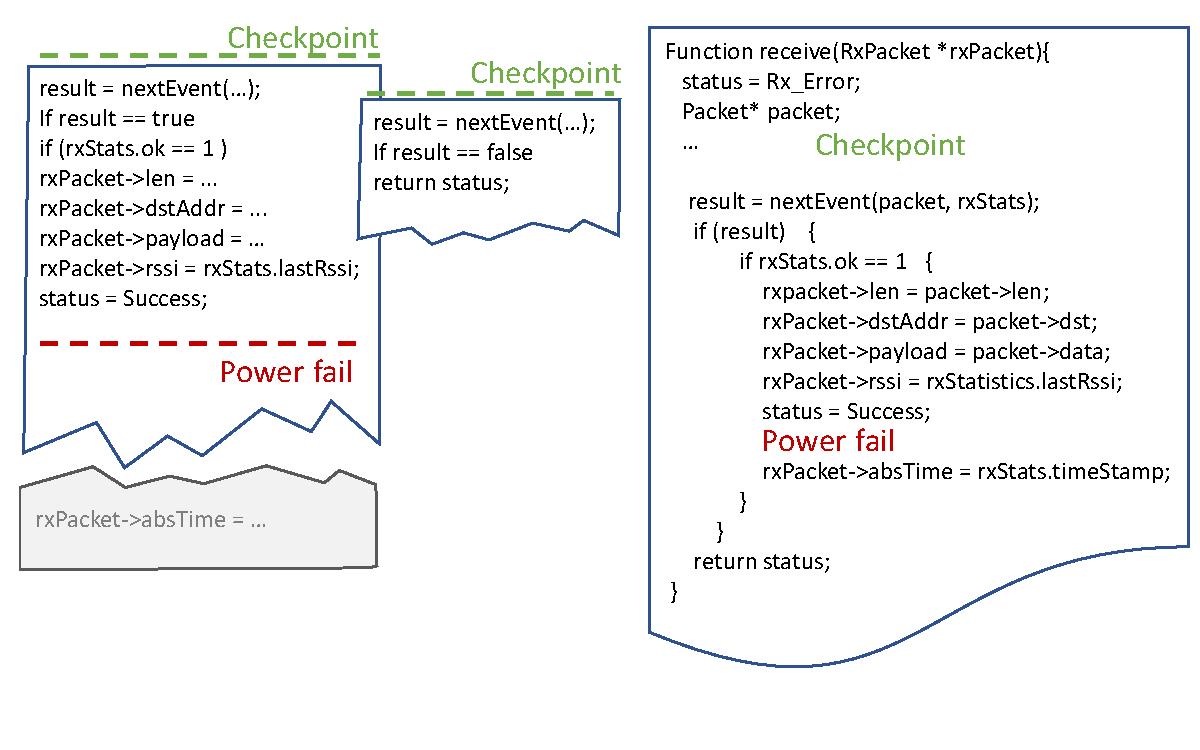
\includegraphics[width=1\columnwidth]{easylinkrx_bug.pdf}
\caption{Bug in RF EasyLink Receiver. Power failing before returning a correctly read packet can cause the status field to be set to success, even if the next event fails. The function will return an incorrect status value, potentially crashing the larger application.}
\label{fig:rf}
\end{figure}